\documentclass{article}
\usepackage[utf8]{inputenc}
\usepackage[letterpaper,margin=1.0in]{geometry}
\usepackage{hyperref}
\usepackage{amsmath,amssymb}
\usepackage[backend=bibtex,sorting=none]{biblatex} % references
\bibliography{library}
\usepackage{graphicx}
\usepackage{subfig}
\usepackage{wrapfig}
\usepackage{titling}
\usepackage{adjustbox}
\usepackage{float}

% Nice latex code display
% http://tex.stackexchange.com/a/173854
\usepackage{tcolorbox}
\tcbuselibrary{minted,skins}
\definecolor{bgcolor}{rgb}{0.95,0.95,0.95}
\newtcblisting{mintcust}[1][]{
  listing engine=minted,
  colback=bgcolor,
  colframe=black!60,
  listing only,
  minted style=colorful,
  minted language=c,
  minted options={linenos=true,numbersep=3mm,texcl=true,#1},
  left=5mm,enhanced,
  overlay={\begin{tcbclipinterior}\fill[black!15] (frame.south west)
            rectangle ([xshift=5mm]frame.north west);\end{tcbclipinterior}}
}



\title{Comparison of Image Convolution on Heterogeneous Architectures}
\author{Patrick Geneva}
\date{December 15, 2017}

\begin{document}


\setlength{\droptitle}{-2cm}
\maketitle

%%%%%%%%%%%%%%%%%%%%%%%%%%%%%%%%%%%%%%%%%%%%%%%%%%%%%%%%%%%%%%%%%%
%%%%%%%%%%%%%%%%%%%%%%%%%%%%%%%%%%%%%%%%%%%%%%%%%%%%%%%%%%%%%%%%%%
%%%%%%%%%%%%%%%%%%%%%%%%%%%%%%%%%%%%%%%%%%%%%%%%%%%%%%%%%%%%%%%%%%
\section{Problem Definition}

We look to investigate the performance differences on different architectures in the application of image convolutions.
Performing convolutions is a common practice in computer vision for apply filters and calculating image gradients.
For example, a filter can be used to blur and image, then calculate its image derivatives to extract key features or edges in the image.
Thus we are motivated to investigate how this building block of many computer vision algorithms performs on different architectures.

\begin{figure}[h]
\centering
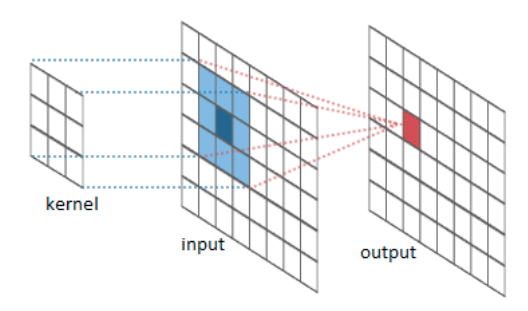
\includegraphics[width=0.5\textwidth]{fig_gen/conv.png}
\caption{Pictorial explanation of how 2D image convolution is applied.}
\end{figure}


To provide a fair comparison all algorithms are implements in C++ and are a ``stripped down'' version of a full algorithm.
We look at a 2D image convolution that is multiplying a small kernel matrix to a larger input image.
Given a pixel location in the input image, the kernel is applied to the surrounding local pixels using element-wise multiplication.
The resulting multiplications are then summed and stored in the final output image.
This process is repeated for each pixel in the incoming image as seen above.
An example result is shown below:


\begin{figure}[H]%
    \centering
    \subfloat[Input image that will have a kernel applied to it]{{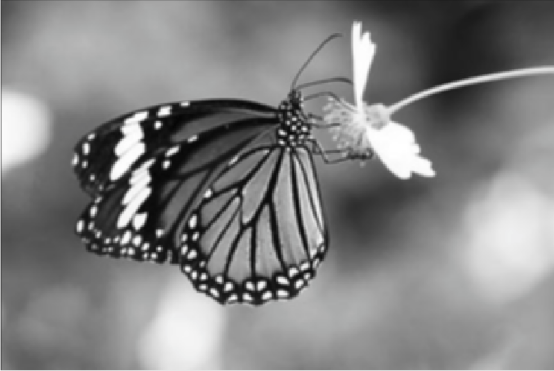
\includegraphics[width=5cm]{fig_gen/input.png} }}%
    \qquad
    \subfloat[Outputted image after convolution with a kernel]{{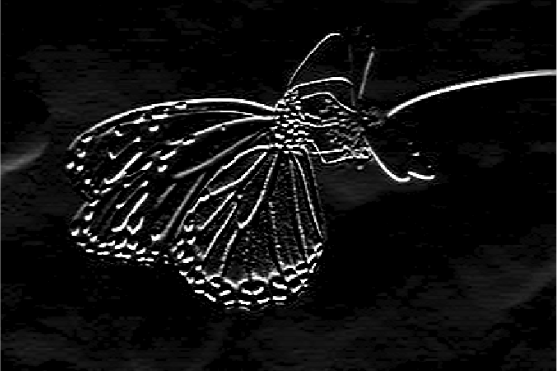
\includegraphics[width=5cm]{fig_gen/output.png} }}%
    %\caption{2 Figures side by side}%
\end{figure}




%%%%%%%%%%%%%%%%%%%%%%%%%%%%%%%%%%%%%%%%%%%%%%%%%%%%%%%%%%%%%%%%%%
%%%%%%%%%%%%%%%%%%%%%%%%%%%%%%%%%%%%%%%%%%%%%%%%%%%%%%%%%%%%%%%%%%
%%%%%%%%%%%%%%%%%%%%%%%%%%%%%%%%%%%%%%%%%%%%%%%%%%%%%%%%%%%%%%%%%%
\section{Convolution Implementations}

In this section we will present simple pseudo code representations of the implemented convolutions.
We will have three different implementations: single threaded, multi-threaded using OpenMP, and GPU accelerated using CUDA.
For each we will present the small changes needed to adapt the base code into its parallelizable format.
We note here that we are capable of parallelizing out code since the outer for loops are independent.

\begin{minted}[frame=lines,framesep=2mm,baselinestretch=1.0,fontsize=\footnotesize,linenos]{c++}
// Loop through in image
for(int i=0; i<rows; ++i) {
    for(int j=0; j<cols; ++j) {
		double sum = 0.0;
		// Sum the image*kernel
		for(int nn=0; nn<krows; ++nn) {
			for(int mm=0; mm<kcols; ++mm){
				int ii = i + nn - krows/2;
				int jj = j + mm - kcols/2;
				sum += imageIn[ii][jj]*kernel[nn][mm];
			}
		}
		// Store the result
		imageOut[i][j] = sum;
	}
}
\end{minted}

The above pseudo code single threaded implementation shows how the based method works.
We loop through all pixels in the input image and for each pixel sum the element-wise multiplication with the given kernel.
We start in the top left of the kernel and move our way row-wise through it.
We then store this sum in the final image out matrix that contains the resulting image (note that we have omitted bound checks and other smaller details for clarity here).

Next we move to multi-thread this code using OpenMP.
It is simple to do so since we have independent loops.
We use the ``collapse'' operator to collapse the two outer loops into a single loop and ask OpenMP to parallelize this code.
We can see below on line 2 the inserted pragma into the C++ code.

\begin{minted}[frame=lines,framesep=2mm,baselinestretch=1.0,fontsize=\footnotesize,linenos,escapeinside=||]{c++}
// Loop through in image
|\textcolor{red}{\textbf{#pragma omp parallel for collapse(2)}}|
for(int i=0; i<rows; ++i) {
	for(int j=0; j<cols; ++j) {
		double sum = 0.0;
		// Sum the image*kernel
		for(int nn=0; nn<krows; ++nn) {
			for(int mm=0; mm<kcols; ++mm){
				int ii = i + nn - krows/2;
				int jj = j + mm - kcols/2;
				sum += imageIn[ii][jj]*kernel[nn][mm];
			}
		}
		// Store the result
		imageOut[i][j] = sum;
	}
}
\end{minted}

To parallelize the code using CUDA we create a kernel that will be launched on the GPU device.
We also note that one could use OpenMP to target the GPU device instead of creating a CUDA kernel.
We launch this kernel in sets of 32x32 blocks and then calculate the needed grid size from the number of pixels needing the operation divided by this 32x32 (1024) threads inside of a single block.
The input image and kernel is first allocated and the copied onto the device.
From there the kernel is launch and the final output matrix is copied back to the host.
Seen below it can be seen that we calculate the i and j pixel locations using the standard thread and block id variables.

\begin{minted}[frame=lines,framesep=2mm,baselinestretch=1.0,fontsize=\footnotesize,linenos,escapeinside=||]{c++}
// Calculate loc from block/thread id
|\textcolor{red}{\textbf{int i = blockIdx.x*blockDim.x + threadIdx.x;}}|
|\textcolor{red}{\textbf{int j = blockIdx.y*blockDim.y + threadIdx.y;}}|

double sum = 0.0;
// Sum the image*kernel
for(int nn=0; nn<krows; ++nn) {
	for(int mm=0; mm<kcols; ++mm){
		int ii = i + nn - krows/2;
		int jj = j + mm - kcols/2;
		sum += imageIn[ii][jj]*kernel[nn][mm];
	}
}

// Store the result
imageOut[i][j] = sum;
\end{minted}

It should be notes that we can accelerate the above code by leveraging shared memory.
All threads use the kernel thus this information can be copied into the local shared memory for all threads to use inside of a block.
We perform that as follows:

\begin{minted}[frame=lines,framesep=2mm,baselinestretch=1.0,fontsize=\footnotesize,linenos,escapeinside=||]{c++}
// Copy to shared memory
__shared__ double skernel[KERNEL_SIZE*KERNEL_SIZE];
// Only have the subset of threads copy to the local memory
if (threadIdx.x < KERNEL_SIZE && threadIdx.y < KERNEL_SIZE) {
      skernel[threadIdx.x*kRows+threadIdx.y] = kernel[threadIdx.x*kRows+threadIdx.y];
}
// Sync so we know we have copied everything
__syncthreads();
\end{minted}



%%%%%%%%%%%%%%%%%%%%%%%%%%%%%%%%%%%%%%%%%%%%%%%%%%%%%%%%%%%%%%%%%%
%%%%%%%%%%%%%%%%%%%%%%%%%%%%%%%%%%%%%%%%%%%%%%%%%%%%%%%%%%%%%%%%%%
%%%%%%%%%%%%%%%%%%%%%%%%%%%%%%%%%%%%%%%%%%%%%%%%%%%%%%%%%%%%%%%%%%
\section{Experiential Results}

To evaluate these different methods we run the code on three different systems.
The hardware specifications can be summarized in the below table.
We run each convolution 25 times and for each calculate the average and deviation each set of trails had.
Additionally for the GPU implementation we record sub-sections of the program to provide an interesting discussion on the distribution of time.

\vspace{2em}
\begin{adjustbox}{center}
\begin{tabular}{r|c|c|c|}
\cline{2-4}
 & \textbf{Thinkpad p51} & \textbf{Desktop \#1} & \textbf{Desktop \#2} \\ \hline
\multicolumn{1}{|r|}{CPU Model} & \begin{tabular}[c]{@{}c@{}}Intel Xeon E3-1505M v6\\ (kaby lake)\end{tabular} & \begin{tabular}[c]{@{}c@{}}AMD FX-8120 Eight-Core Processor\\ (fx-series)\end{tabular} & \begin{tabular}[c]{@{}c@{}}Intel Core i7-7800X\\ (skylake)\end{tabular} \\ \hline
\multicolumn{1}{|r|}{CPU Cores} & 4 real, 4 virt & 8 real & 6 real, 6 virt \\ \hline
\multicolumn{1}{|r|}{CPU Clock Speed (GHz)} & 3.0, 4.0 boost & 3.1, 4.0 boost & 3.5, 4.0 boost \\ \hline
\multicolumn{1}{|r|}{GPU Model} & \begin{tabular}[c]{@{}c@{}}Quadro M2200\\ (maxwell)\end{tabular} & \begin{tabular}[c]{@{}c@{}}GeForce GTX 970\\ (maxwell)\end{tabular} & \begin{tabular}[c]{@{}c@{}}GeForce GTX 1080 Ti\\ (pascal)\end{tabular} \\ \hline
\multicolumn{1}{|r|}{GPU Clock Speed (GHz)} & 1.04 & 1.33 & 1.67 \\ \hline
\multicolumn{1}{|r|}{GPU Memory (GB)} & 4 & 4 & 11 \\ \hline
\multicolumn{1}{|r|}{GPU CUDA Cores} & 1024 (8 MP) & 1664 (13 MP) & 3584 (28 MP) \\ \hline
\end{tabular}
\end{adjustbox}



\begin{figure}[H]
\centering
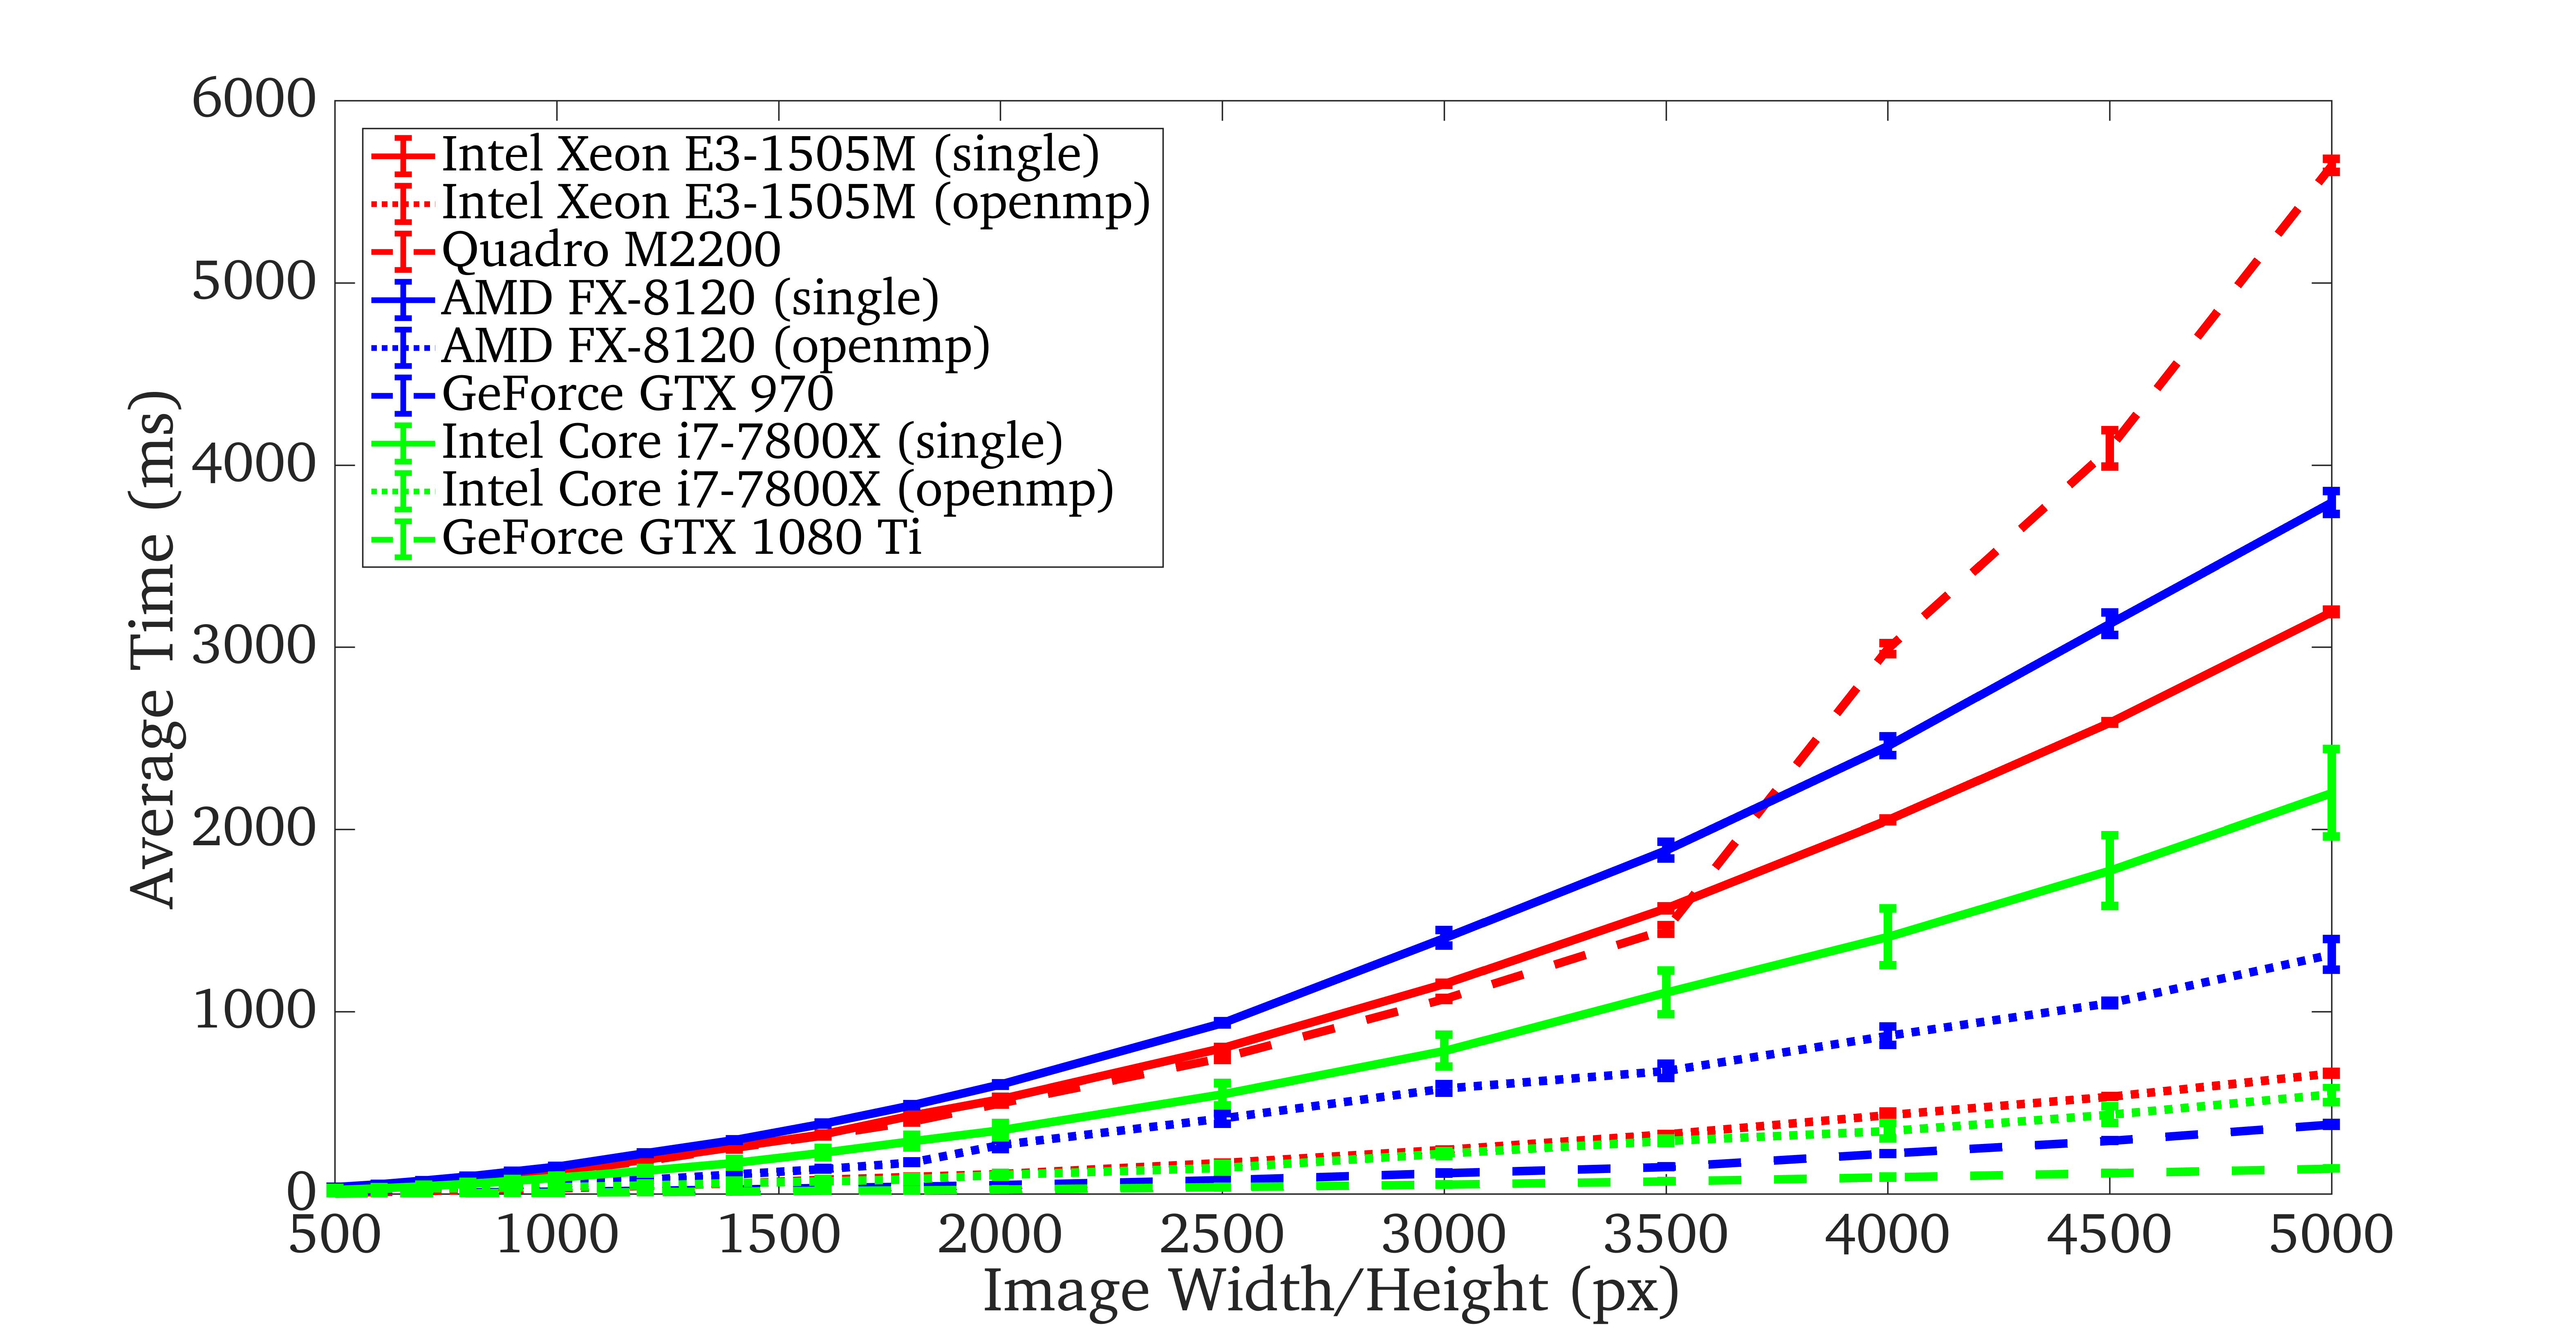
\includegraphics[width=0.8\textwidth]{fig_results/plot_times_sys.png}
\caption{Execution times in milliseconds with deviations for each system show in different colors.}
\end{figure}

\begin{figure}[H]
\centering
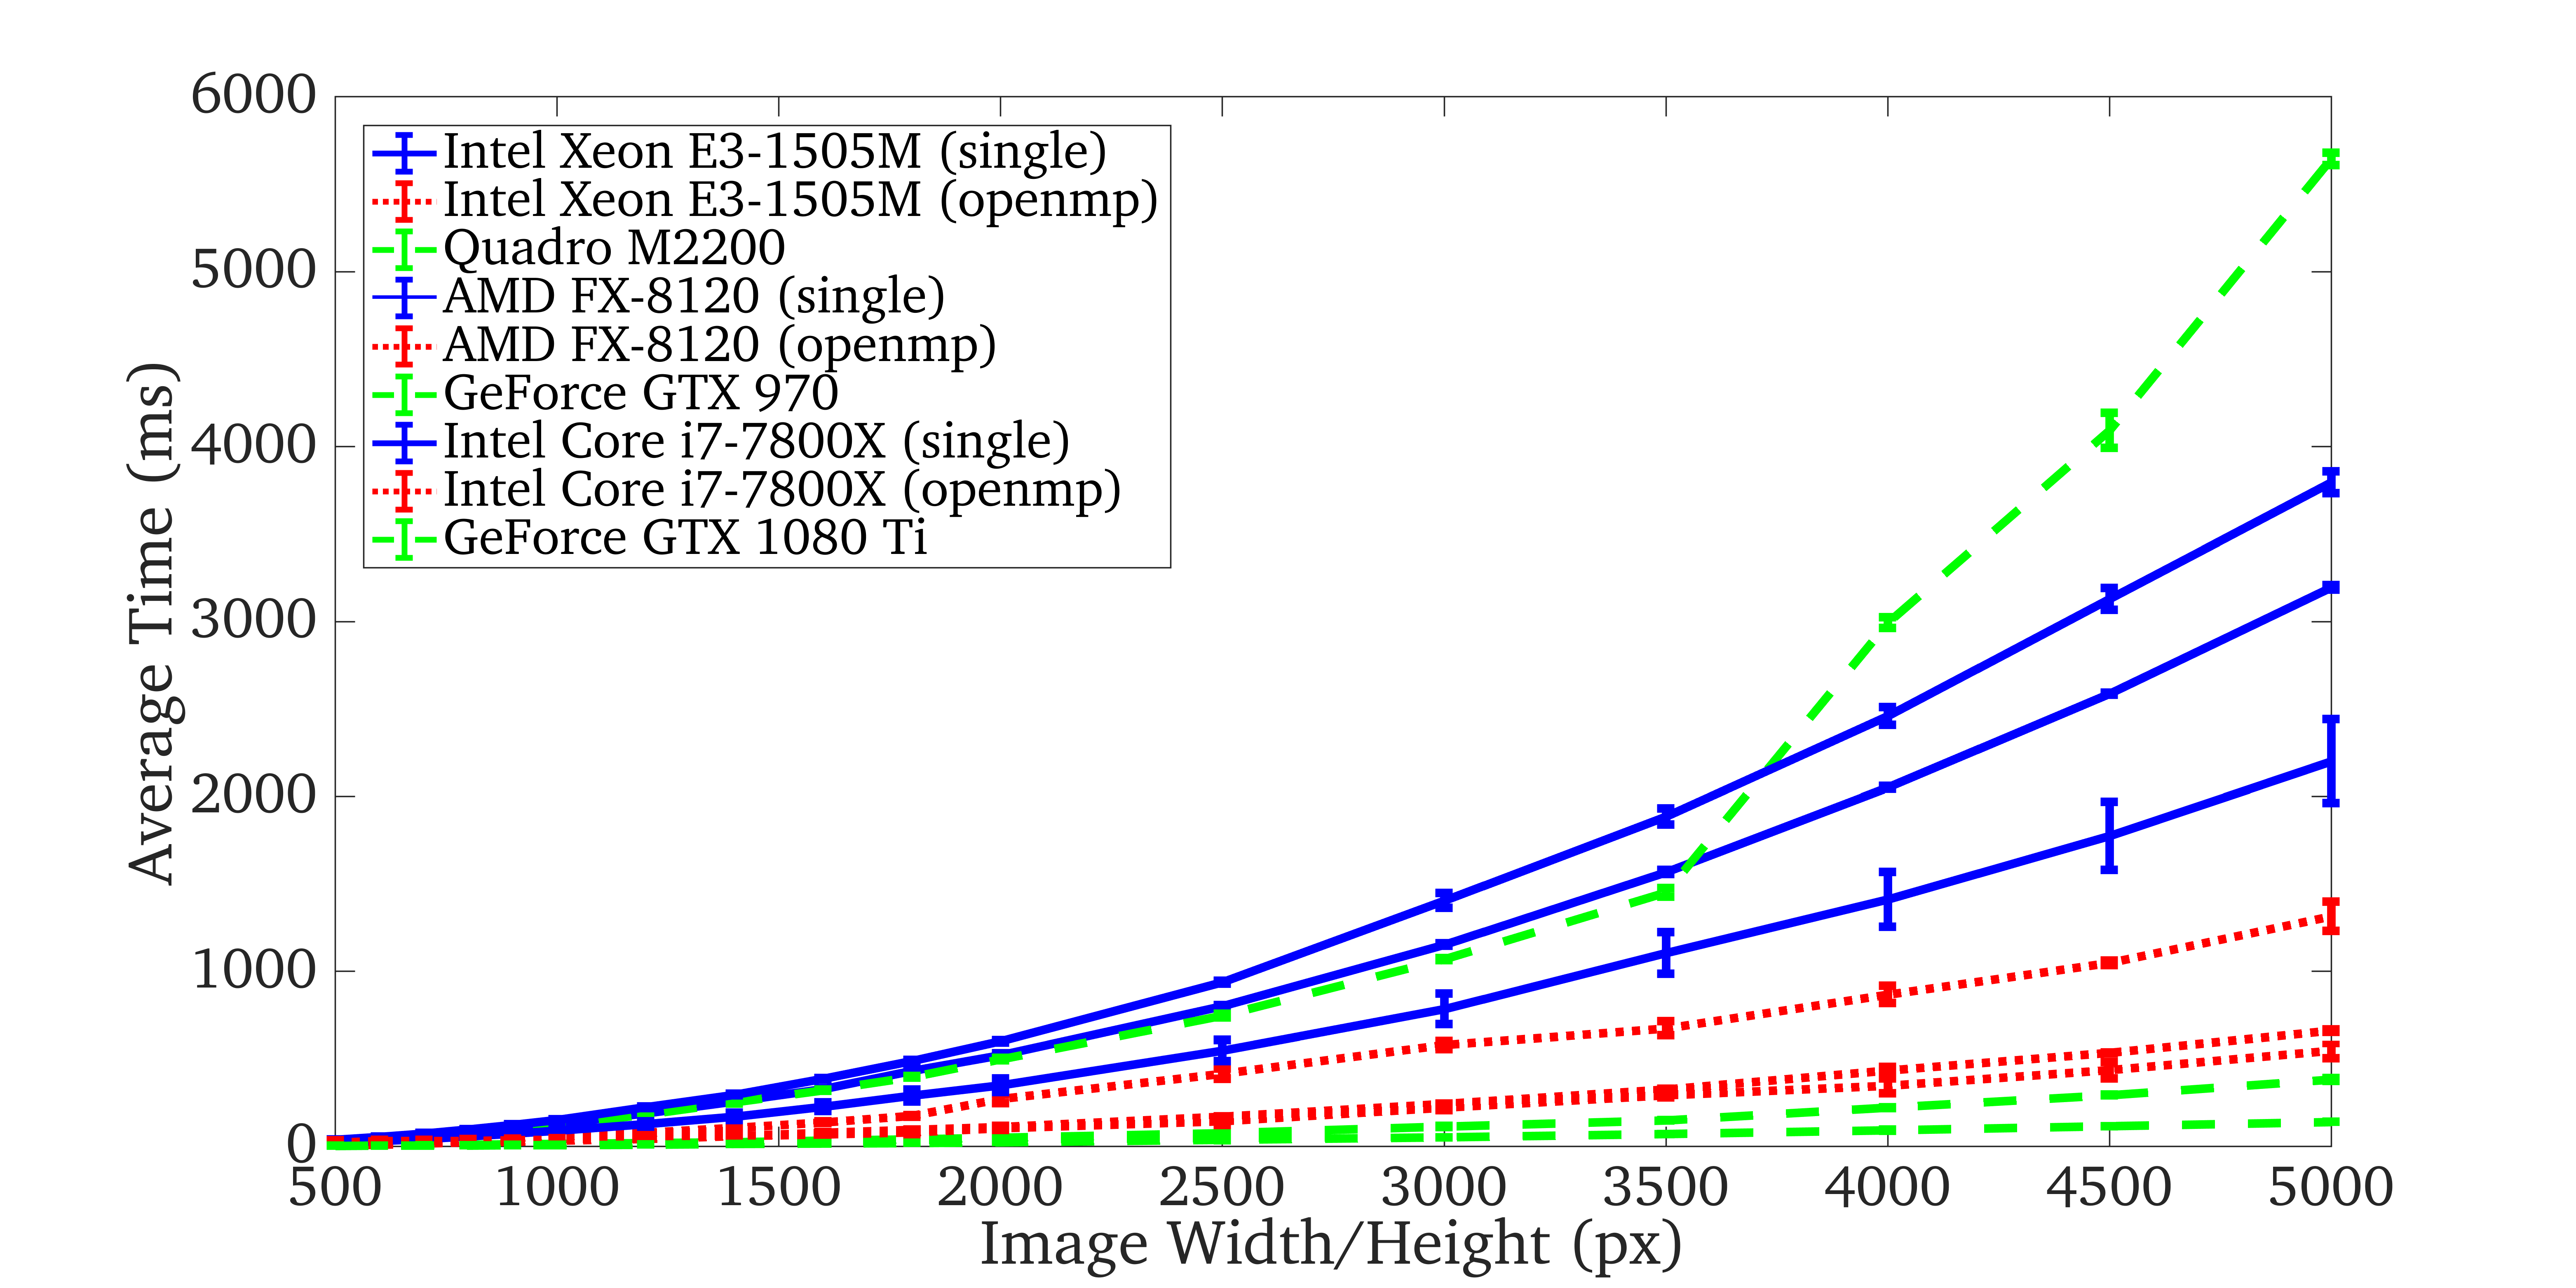
\includegraphics[width=0.8\textwidth]{fig_results/plot_times_type.png}
\caption{Execution times in milliseconds with deviations for each type of optimization. CPUs are shown in blue, OpenMP multi-threading shown in red and GPU CUDA implementations shown in green.}
\end{figure}


\begin{figure}[H]%
    \centering
    \subfloat[Nvidia Quadro M2200 GPU execution time splits.]{{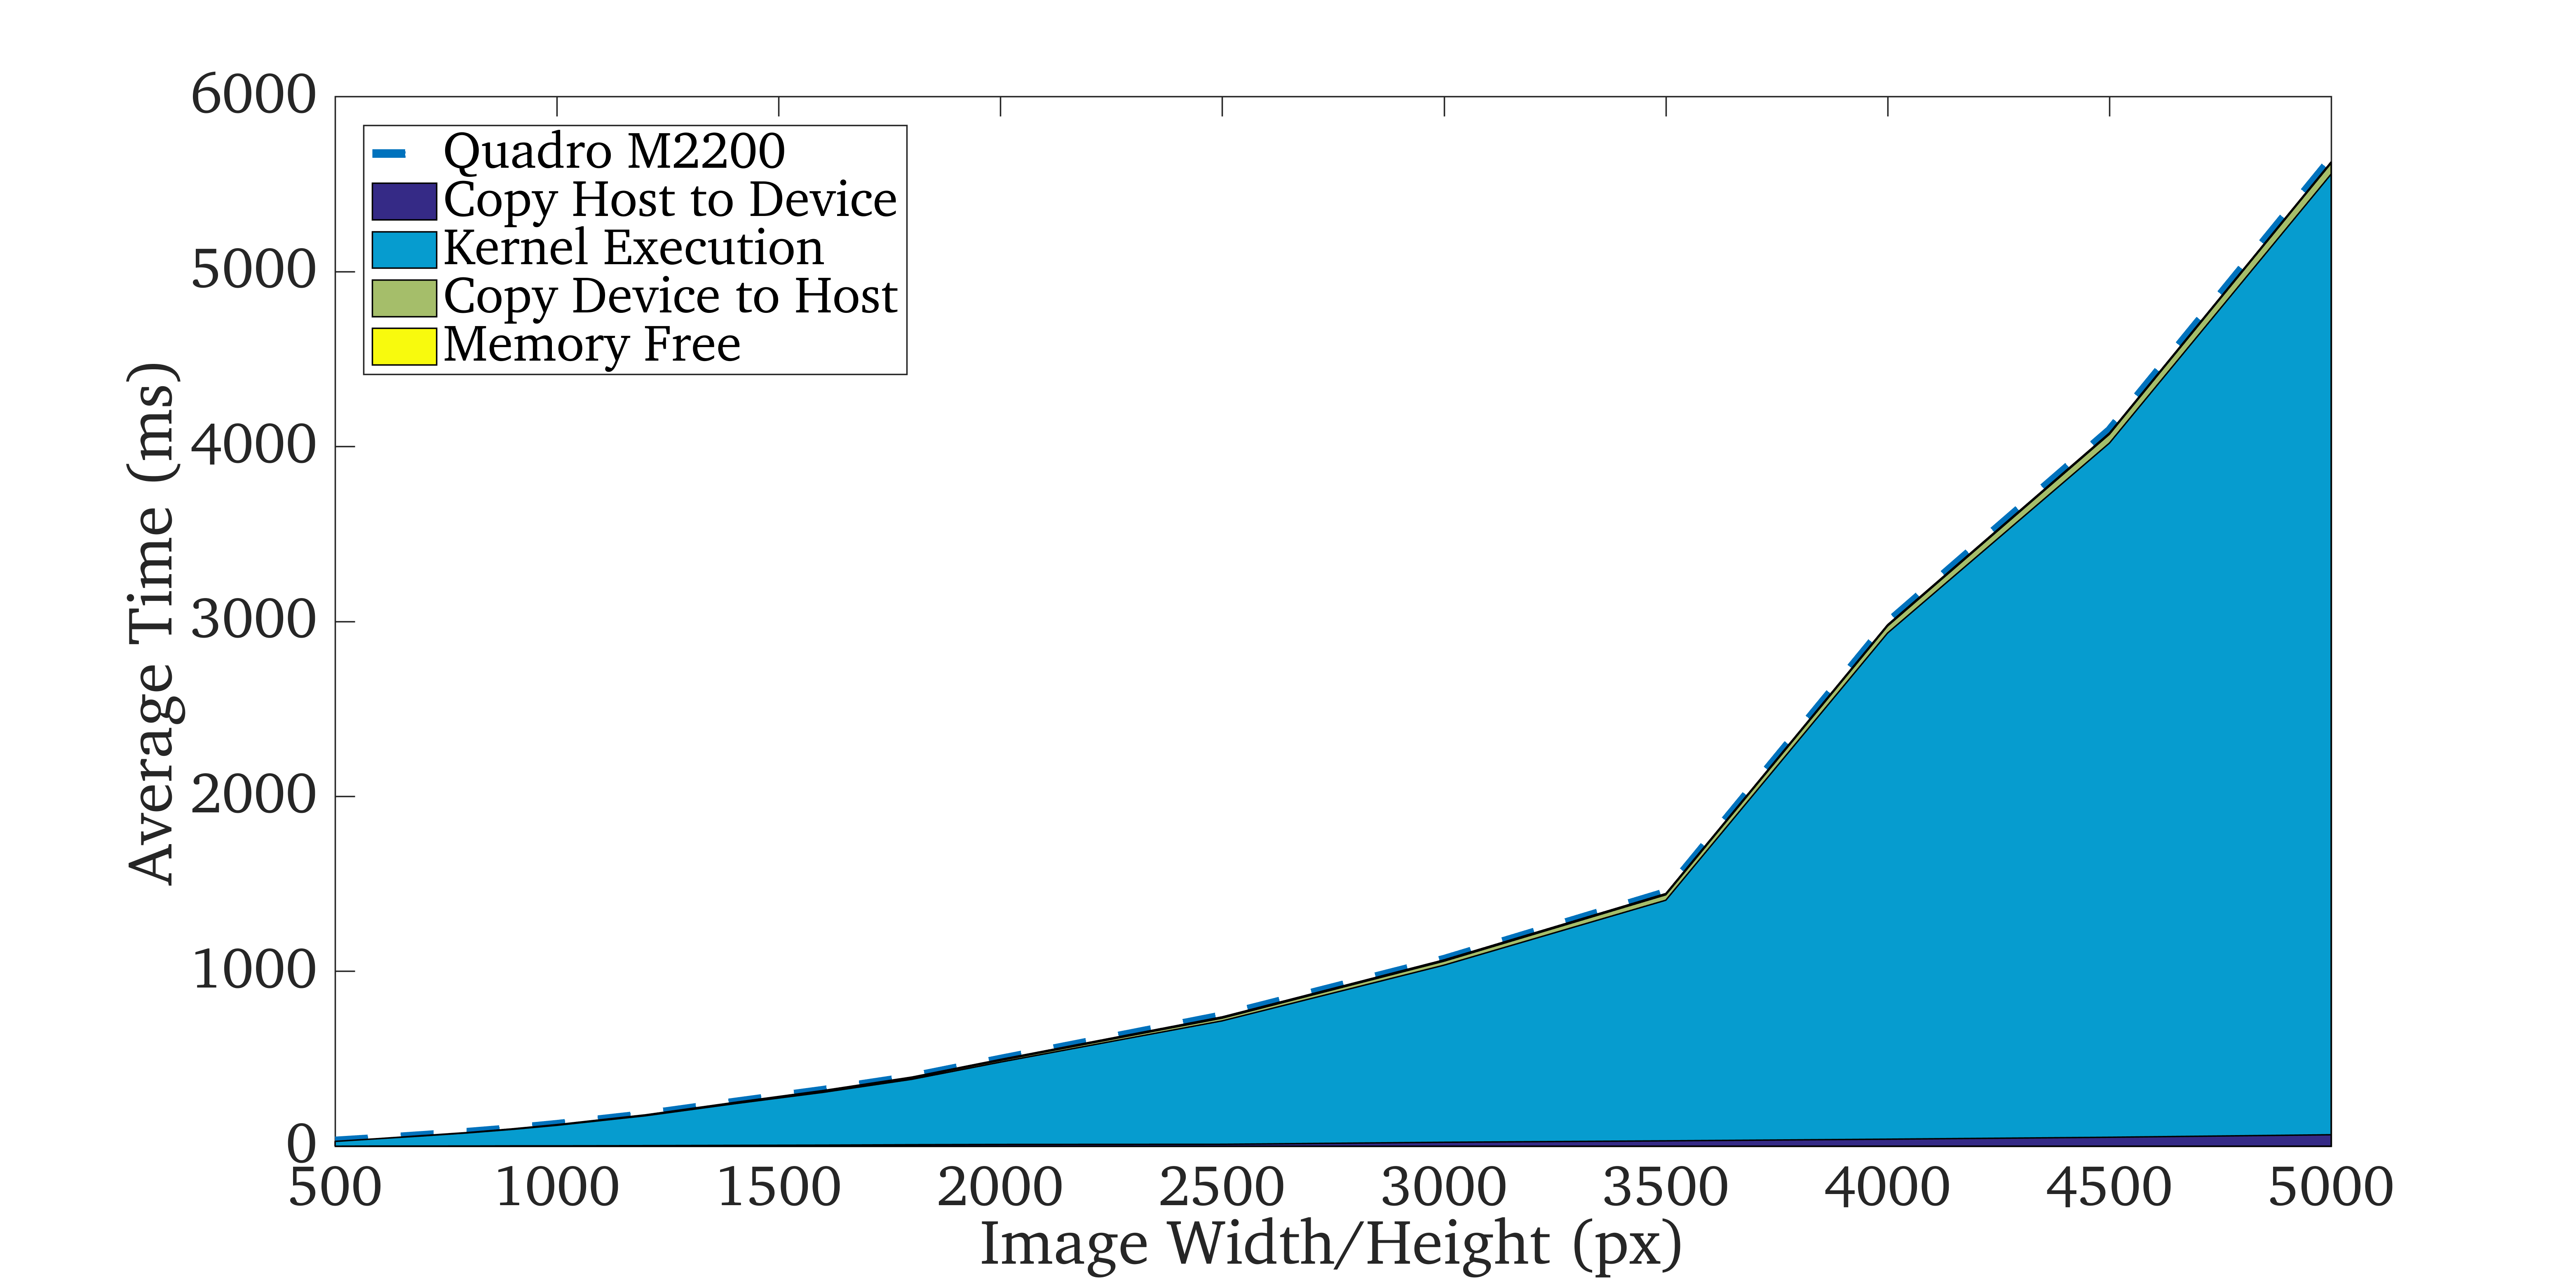
\includegraphics[width=0.45\linewidth]{fig_results/plot_gpusplit_1_M2200.png} }}%
    \qquad
    \subfloat[Nvidia GTX 970 GPU execution time splits.]{{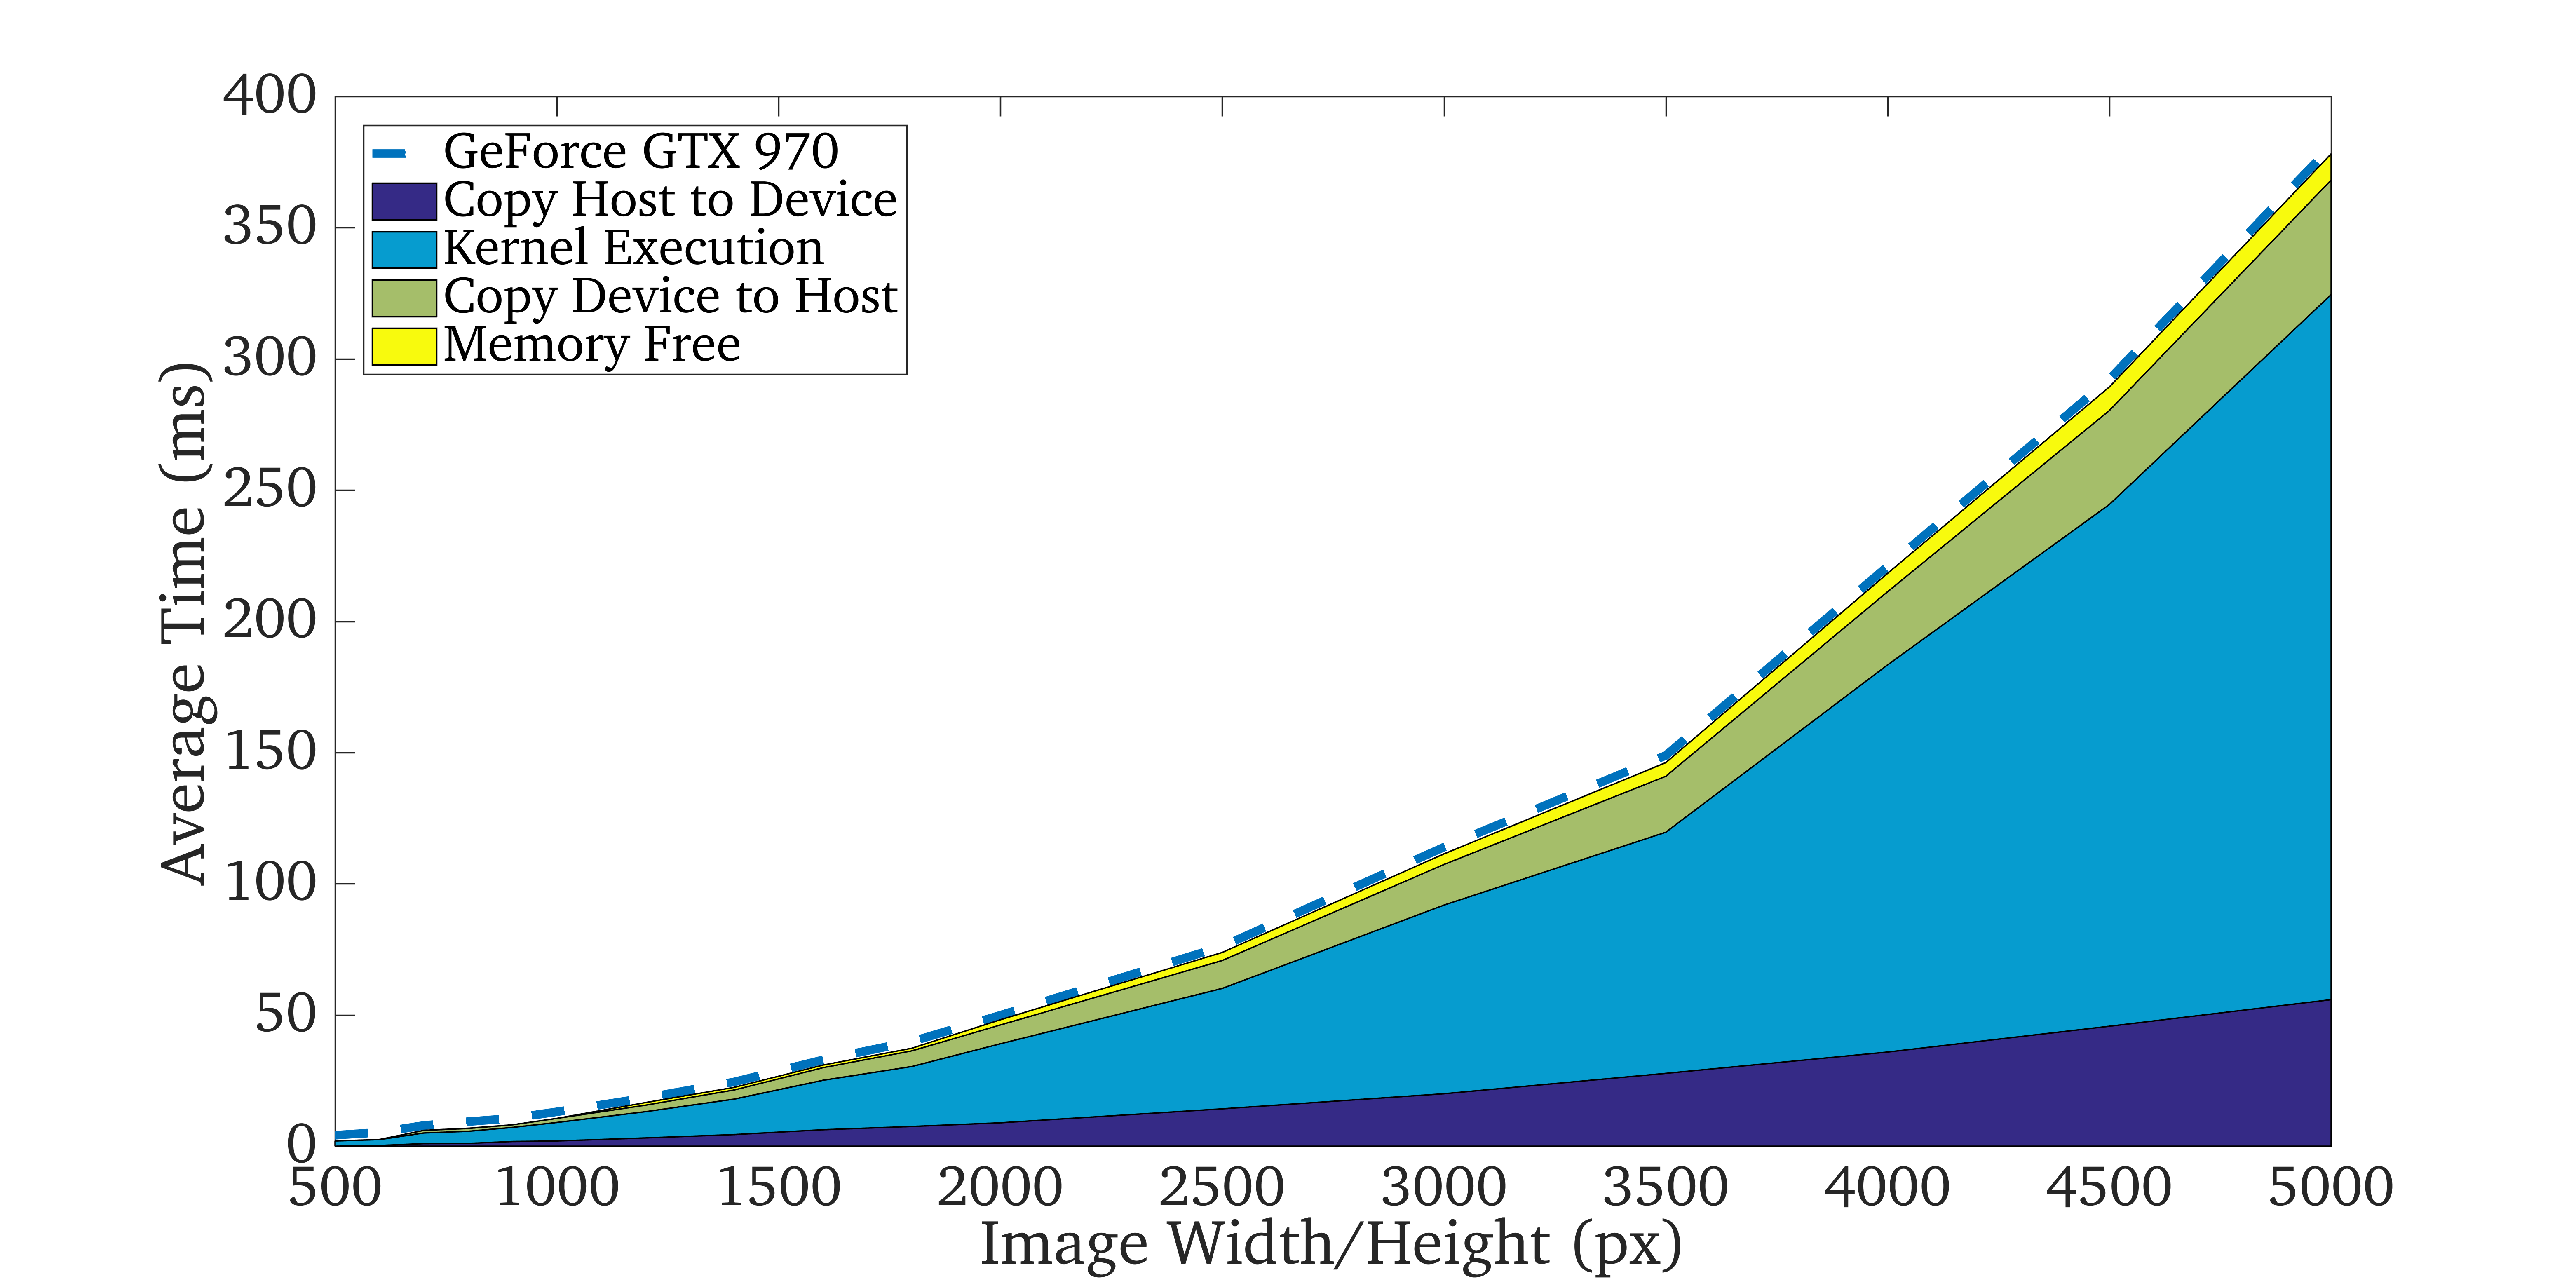
\includegraphics[width=0.45\linewidth]{fig_results/plot_gpusplit_2_GTX970.png} }}%
\end{figure}

\begin{figure}[H]
\centering
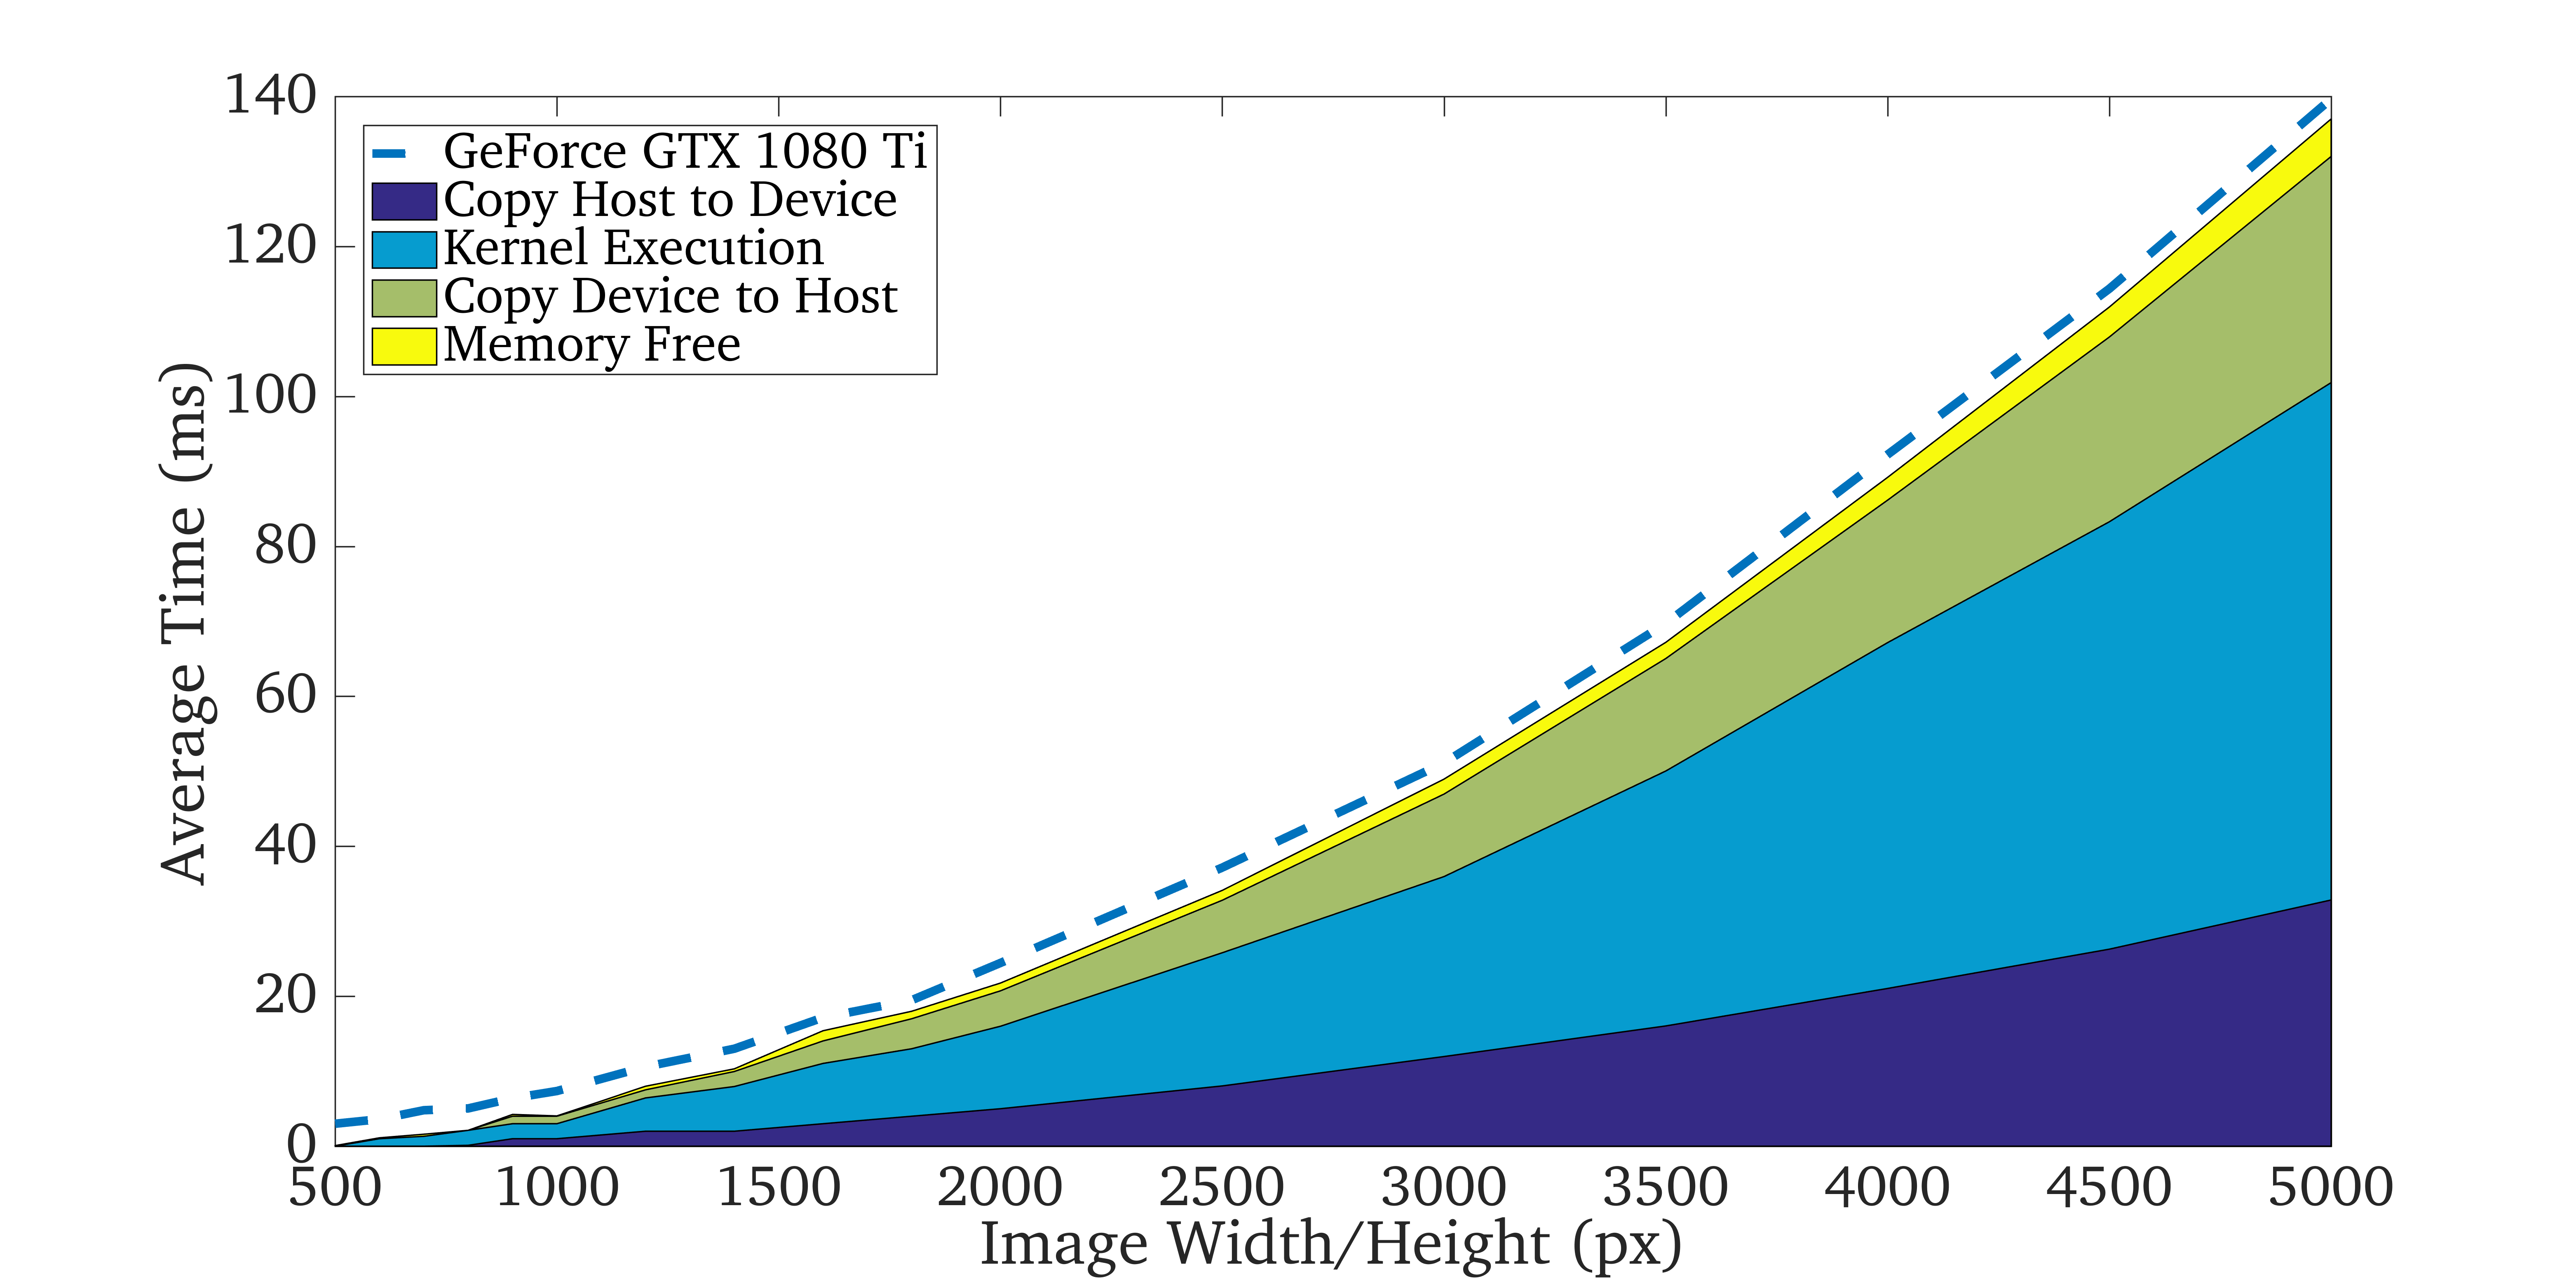
\includegraphics[width=0.45\linewidth]{fig_results/plot_gpusplit_3_GTX1080ti.png}
\caption{Nvidia GTX 1080ti GPU execution time splits.}
\end{figure}


%%%%%%%%%%%%%%%%%%%%%%%%%%%%%%%%%%%%%%%%%%%%%%%%%%%%%%%%%%%%%%%%%%
%%%%%%%%%%%%%%%%%%%%%%%%%%%%%%%%%%%%%%%%%%%%%%%%%%%%%%%%%%%%%%%%%%
%%%%%%%%%%%%%%%%%%%%%%%%%%%%%%%%%%%%%%%%%%%%%%%%%%%%%%%%%%%%%%%%%%
\section{Discussion}

Seen above we can clearly see the speedup due to both multi-threading and parallelization onto a GPU.
It is interesting to note that the Quadro M2200 did not scale that well with the increased size of the image.
This is likely due to the smaller number of CUDA cores and the clock speed on the mobile laptop platform.
We can also see in the above time split breakdowns for the Quadro M2200 that the kernel execution is what takes the majority of the execution time.
We can also see that the GTX 1080ti has a more even split between the components that contribute to its execution time, suggesting that it can both process faster but also more data.


\begin{figure}[H]
\centering
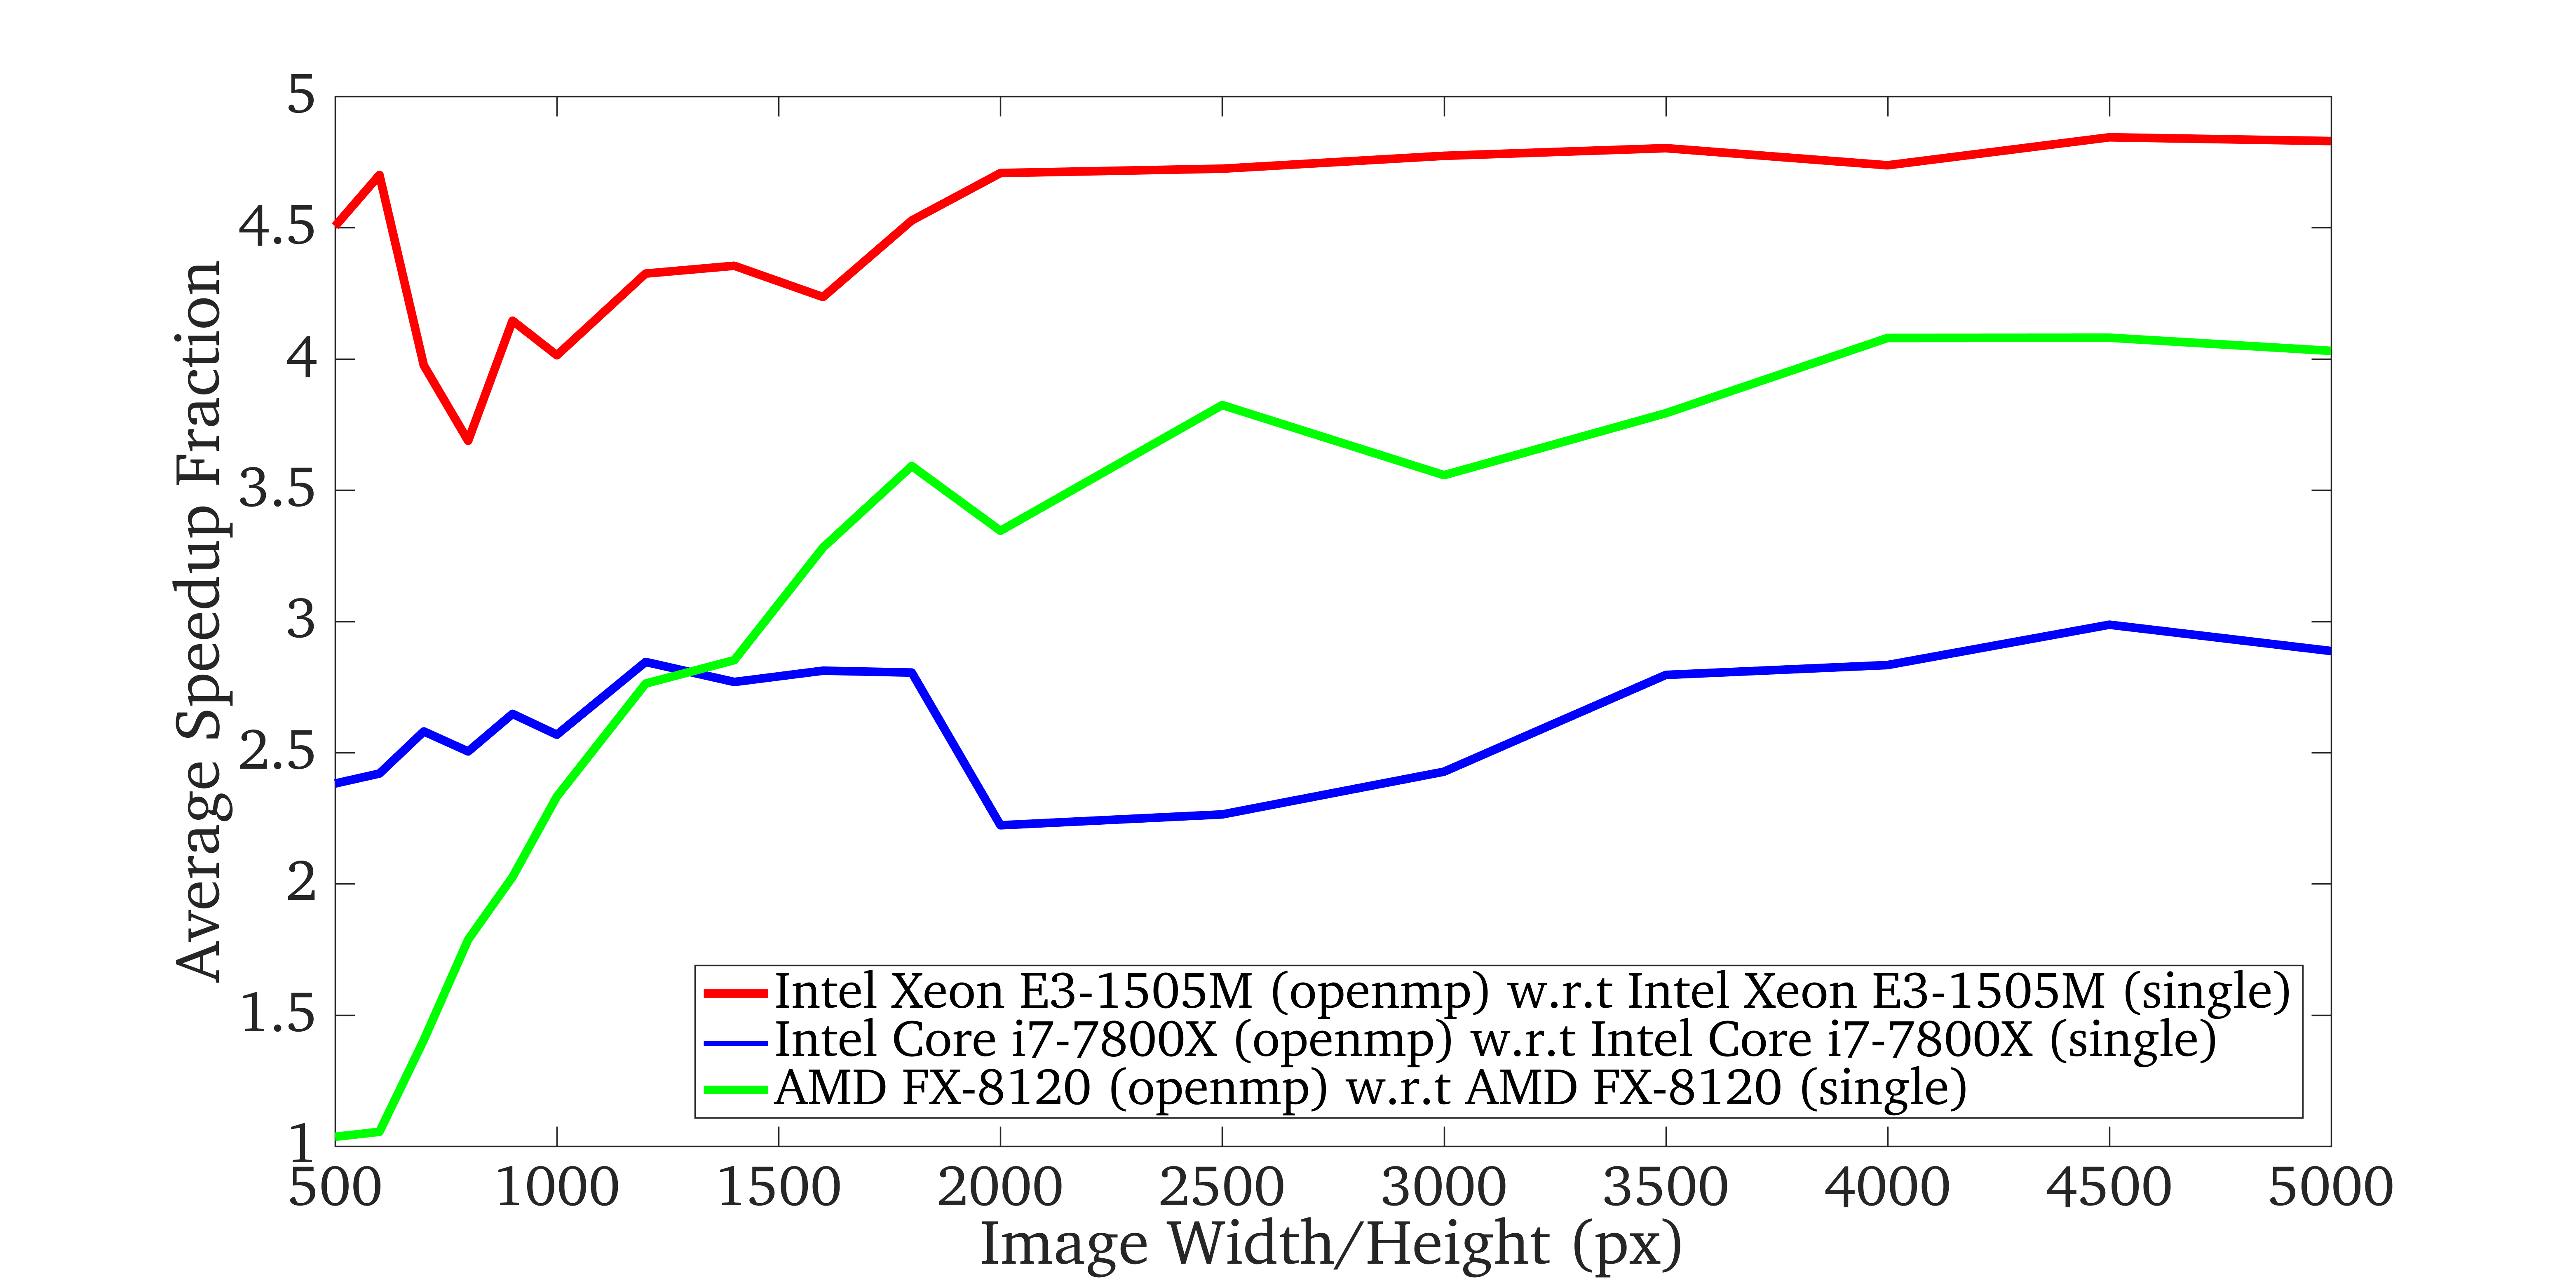
\includegraphics[width=0.8\textwidth]{fig_results/plot_speedup_cpus.png}
\caption{Speedup going from a single threaded program to a multi-threaded program using OpenMP.}
\end{figure}

\begin{figure}[H]
\centering
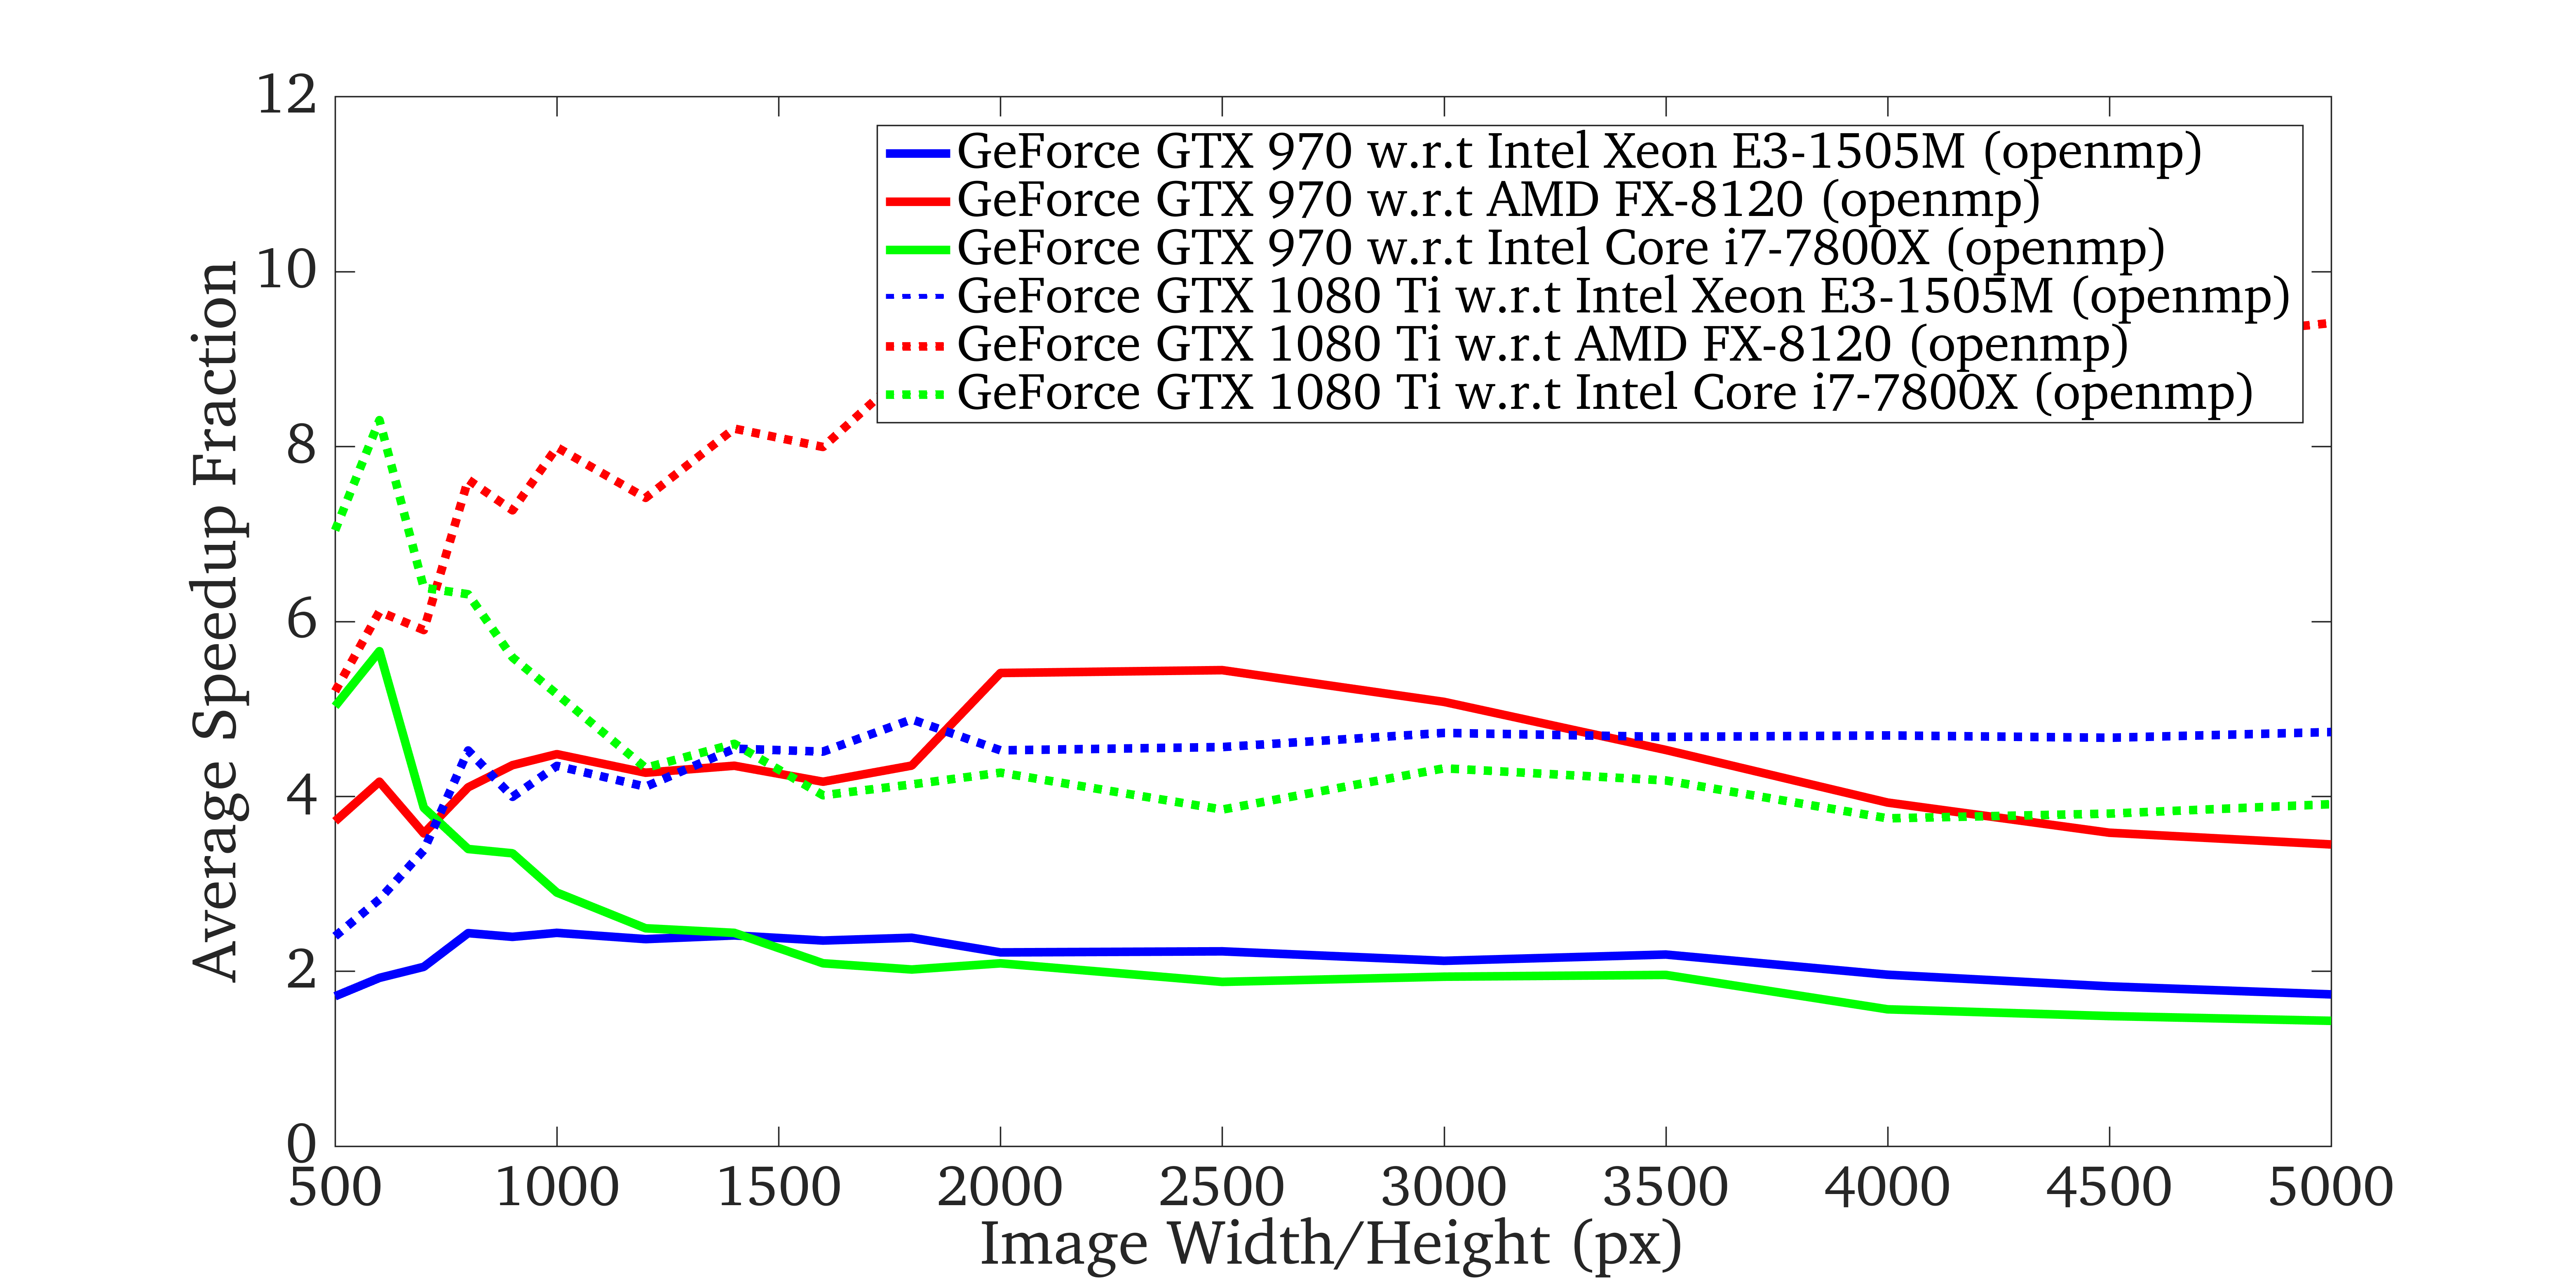
\includegraphics[width=0.8\textwidth]{fig_results/plot_speedup_gpus.png}
\caption{Speedup going from a multi-threaded program using OpenMP to a GPU accelerated program using a CUDA kernel implementation.}
\end{figure}


\noindent
Looking at the speedup from taking a single threaded program and using OpenMP to multithread it, we can see that the Intel Xeon had an massive speedup of x4.5.
It is interesting to see that the AMD FX-8120 does not have a constant speedup and instead only exhibits speedup when the image is greater then 1000x1000 pixels.
This is likely due to the thread overhead being greater then the computations done by each thread (a thread calculates a convolution for a single pixel).
When looking at the speedup when going from a multithreaded version to a GPU CUDA accelerated version we can see that there is a large speedup between 2-4x.
We can see that the newer 1080ti care has a 2x speedup relative to GTX 970.
While this is an expected result, we want to note that if one has a Xeon or i7 one can simply multithread using OpenMP and will only miss out on a 2x speedup if it was parallelize on the GPU.

In conclusion, we see that the parallelization of image convolution allows for a speedup of the over all execution time.
We also show that in newer GPU units the kernel execution time on smaller problems is a smaller fraction relative to the transfer times.
Finally we note that enabling multithreading on a CPU will give you the highest ``value proposition'' if you can sacrifice a 2x-3x speedup out of a total of 6x speedup.
This is especially true if the processor being used is a Intel Xeon.



\end{document}
